\documentclass[tikz]{standalone}
\usepackage{amsmath}
\usetikzlibrary{matrix}
%% EXTRA_TIKZ_PREAMBLE_CODE %%
\begin{document}
%% TIKZ_CODE %%
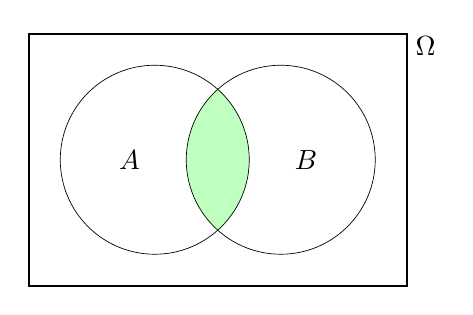
\begin{tikzpicture}[line width=0.25pt, scale=0.8]
\begin{scope} 
	\clip (4,2) circle (1.5); 
	\fill  [green!25] (2,2) circle (1.5); 
\end{scope}

\draw[thick] (0,0) rectangle (6,4);
\draw (6.3,3.8) node {$\Omega$};
\draw (2,2) circle (1.5); \draw (1.6,2.0) node {$A$};
\draw (4,2) circle (1.5); \draw (4.4,2.0) node {$B$};

\end{tikzpicture}
\end{document}
